%The background should set the project into context by motivating the subject matter and relating it to existing published work. The background will include a critical evaluation of the existing literature in the area in which your project work is based and should lead the reader to understand how your work is motivated by and related to existing work.
\chapter{Background research}
This chapter aims to introduce some concepts surrounding our problem domain, which to help the reader to understand and follow easier the following more technical chapters. I also present a review of the related work that has been done in this area. The below sections look at some of the key aspects and problems that arise. I then conclude by providing a number of alternative methods for solving our problem.

%Explain Curtailments (short turning) - reasons for this are: delays, planned roadworks or events, insufficient layover, improve overall realiability of the service fill gaps, prevent breaches - drivers hours regulation
%Bus bunching 
\section{London Bus Network}
London bus network is one of the most advanced and renowned in the world. It runs 24 hours and it is extensive and frequent. Every route in the network is tendered to different bus company operator \cite{busTendering}. These operators agree with TFL that the routes they are operating would be served either according to a predefined fixed schedule (e.g. a bus stop need to be served at 1pm, 3pm etc.)or on a headway (e.g. a bus stop need to be served every 5 minutes). However under different circumstances some delays occurring on a given route are beyond the control of the different bus operator companies. A simple example could be a burst water/gas pipe on a street used by a bus route or any other incident (even terrorist attacks \cite{centreComm}) and even simply a severe congestion. In situations like this bus operators have no authority or power to overcome such problems on their own. They can only ask CentreComm to intervene. CentreComm can do so by for example implementing a short/long term diversions or curtailments (short turning) some of the buses on the affected routes.

Buses in the network can be classified by multiple factors, however for the purpose of this report the main distinction we need to consider are high and low frequency bus routes. High frequency routes are routes where there are 5 or more buses per hour attending a given bus stop. Low frequency routes are those that have 4 or less buses alighting at a stop.
\section{CentreComm}
CentreComm is TFL's emergency command and control room responsible for all public buses in London. It is has been in operation for more than 30 years \cite{centreComm} and it employs a dedicated
team of professionals who work 24 hours 364 days in the year. They are dealing with more than a 1000 calls on a daily basis. The majority of these calls come from bus drivers or bus company operators regarding problems and incidents happening within the bus network. CentreComm staff implement planned long and short term changes in the bus network in response to different events taking place in the capital (including the 2012 Olympics). They are also responsible for reacting in real time to any unexpected and unpredicted changes and disruptions, maintaining the smooth, reliable and sage operation of London busy bus network.

London bus network consists of around 680 bus routes operated by more than 8000 buses \cite{glads}. Each of this buses is equipped with state of the art iBus system to help monitor and manage this enormous fleet. CentreComm's way of operation has been transformed beyond recognition since it has first opened and today. It started more than 30 years ago \cite{centreComm} and it consisted of a couple of operators equipped with two way radios and pen and papers. Today CentreComm operators make use of numerous screens each displaying interactive maps (displaying each bus location) and CCTV cameras in real-time. However there is still a lot of room for automation and improvement in their way of operation in order to effectively and efficiently maintain the growing bus network.

%CentreComm is not responsible for the fleet management as mentioned above. The emergency control and command room comes into place when there are planned or unplanned events affecting the bus network which need to be taken care of. They are responsible in assisting the bus drivers and bus company operators to manage their schedules when there are events which are beyond their control.
%CentreComm is not responsible for the fleet management as this is contracted to the bus operators which are responsible for maintaining reliable service according to agreed contracts. The emergency control room comes in place when there are planned or unplanned events which disrupt the transport network. They are also responsible for helping the bus operators once they cannot maintain the service they are responsible for due to traffic congestion or other issues which are beyond their control. However currently CentreComm relies on the bus drivers and bus operators for letting them know of such cases as they do not have a system which to signal them about these issues. All the information they need is there and they have access to it however they do not have the resources to manually monitor each of the 8000+ buses.
\section{iBus AVL}
Automatic vehicle location systems make use of the Global Positioning System (GPS) to enable the remote (using the internet) tracking of the locations of the vehicles in a given fleet. This system combines a number of technologies including GPS, cellular communications and more with the goal of improving and cutting the cost of fleet management. 

All of London buses operating on the TFL bus network have been equipped with state of the art and award wining \cite{ibusAward} AVL system named iBus \cite{ibus}. This system has opened a range of new applications that could be built on top of it using the information that is made available. The iBus system consist of a number of computer and communication systems, sensors and transmitters as described in \cite{Hounsell201276} and \cite{eps354267}.
One of the key components of the system on-board unit (OBU) which mounted on each of
buses in the TFL bus fleet and consists of a computational unit connected to
sensors and GPS transmitters (see figure 1 below taken from \cite{Hounsell201276}). 
\begin{figure}[ht!]
\centering
	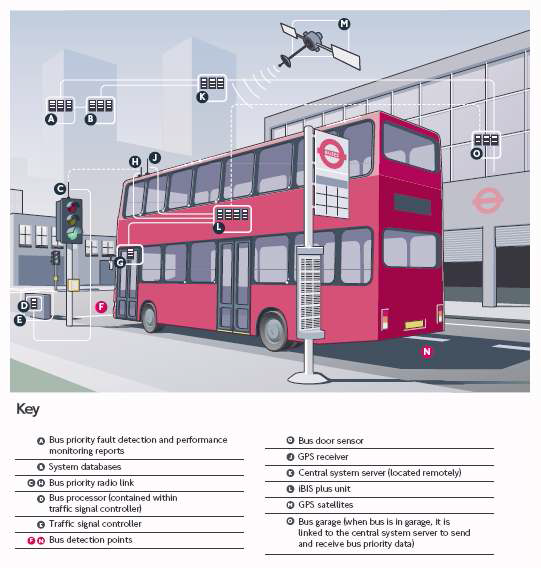
\includegraphics[scale=0.8]{Figures/iBus.png}
\caption{Overview of iBus System (Source: Transport for London, 2006a) \label{overflow}}
\end{figure}
This OBU is responsible for a number of tasks including a regular (approximately every 30 seconds) transmission of the bus location. This information is currently used by the different bus operators for fleet management as well as by CentreComm for real-time monitoring of the buses and their locations. There are have been a number of other applications and systems that have been implemented and put in to use as a result of the data that is generated by the iBus AVL. Some examples include Countdown (real-time passenger information), improved bus priority at traffic signals and more \cite{Hounsell201276}. This has led to improved and more affordable transport service.

CentreComm operators have access to an online system showing each bus location in the network on a map in real-time. This system allows them to see whether a given bus is behind, ahead or on time according to its schedule. However this does not show or alert the control room staff if a bus or a route is disrupted. Control room staff also can see when was a given bus expected to arrive at a given bus stop and when it actually arrived, but this again is only per individual bus. Currently the work-flow is such that CentreComm need to go and analyse all this information manually (once bus drivers or bus company operator have contacted/alerted the control room) in order to figure out if a there is a problem and how severe it is. This is very inefficient, tedious and error prone process. Here is where our project comes into place to address the lack of preprocessed information.

\section{Related Work}
Most of the research that has been done focuses on predicting the bus arrival time. Also most of the related work that I have been able to find focusses on non urban environments or non real-time analysis. Urban environments are complex and unpredictable due to their nature itself. In densely populated areas the bus could skip sending its GPS coordinates due to weak signal (e.g. due to obstruction of tall buildings).

Traffic flow in urban areas is influenced by many factors. One of those is general congestion others include passenger usage (dwell time), weather and others.

According to my knowledge and up to date I have not been able to find any similar research to do with detecting disruptions in a bus network. The literature is full of discussions and approaches for predicting the bus travel and arrival times, but there is none to address the issue of automatic/computerised detection of disruptions in a given bus network or fleet of vehicles is disrupted based on some underlying schedule or metrics.

There is also a lot of research to address the issues around bus prioritisation at traffic signals and junctions [REFERENCE SOME PAPER].

With the increased use of AVL systems for different fleets a number of studies have emerged which tries to use this vehicles as probes for detecting traffic congestion in the network [REFERENCE -Statistical Modelling and Analysis of Sparse Bus Probe Data in Urban Areas]. This research is most closely related to our problem as we are looking to identify route or sections which are disrupted beyond the control of individual bus operator companies. This would most often mean a severe traffic congestion or incident. If there is an incident (e.g. flat tire, customer incident etc.) which is one of occurrence which has affected only a single bus this should not be detected. As this should not be brought to the attention to CentreComm unless it is having a significant impact on the rest of the service or network.

Problems:
The bus could have started the journey ahead of schedule and thus to intentionally be losing time.
The buses could curtail anywhere on a route without notification
The buses could be diverted (this could be short term or long term) it can also be for few stops or it could be a longer diversion.

\section{Approaches}
In the literature we could find different classification of the approaches (models) for predicting bus travel time \cite{surveyAIApplications}. According to \cite{urbanBusArrivalTimeCompModels} we could classify them into four computational models:
\begin{itemize}
	\item Based on historical data
	\item Statistical 
	\item Kalman Filtering 
	\item Machine Learning
\end{itemize}
	\subsection{Statistical}
	%Time series Analysis
Time series is a sequence of data reading taken during successive time intervals. Time series analysis is performed on time series data in order to extract some meaningful statistics from the data. In addition to the time series analysis time series forecasting could also be performed to come up with a prediction for the next period in time based on what has been observed in the past. In our problem this would mean having a number of bus readings we could analyse them and come up with prediction of what would be state in the next point in time. However for our prototype we are mostly concerned with the actual state rather than predicting the future. Forecasting in our problem domain is complex and unpredictable due to the constraints and characteristics of the environment as described above.

		\subsubsection{Simple moving average}
		Simple arithmetic moving average is calculated by adding all the observations for a given period of time and dividing this sum by the total number of observations.
		\subsubsection{Weighted moving average}
		\subsubsection{Exponential moving average}
		\subsection{Peak detection}
		\subsection{Autoregressive moving average}
		
	\subsection{Machine learning}
	
	\subsection{Historical Data}
	
	\subsection{Hybrid}
	
\section{Summary}